\documentclass[10pt]{article}
\usepackage{icmlko}

\icmlmeta{IP 파운데이션 월드모델}{88}{에폭이 늘수록 팝업만 잘 맞혔다}{낙관 편향의 출처를 둘로 갈랐다 --- 학습 시간과 도메인별 머리}

\begin{document}

\twocolumn[
\icmlheader

\begin{abstract}
노트 87이 노트 86의 헤드라인을 철회하며 낙관 편향이 도메인 크기와 $r=-$0.857로
붙는다고 했다. 출처를 갈랐다. \textbf{첫째, 학습 시간이다} --- 팝업(75건)의
편향이 100에폭에서 $+$0.010인데 700에폭에서 \textbf{$+$0.570}이다. 아이돌(81건)도
$+$0.096$\to+$0.512다. 그런데 모바일(2,000건)은 $+$0.003$\to+$0.011로 거의 안
는다. \textbf{작은 도메인에서는 학습 시간이 곧 편향이다.} 노트 85 · 86이 쓴
400에폭에서 팝업 편향이 $+$0.375였고 노트 87이 관측한 $+$0.384와 맞는다.
\textbf{둘째, 도메인별 머리다} --- 머리를 공유로 바꾸면 평균 편향이 $+$0.0624에서
\textbf{$+$0.0296}으로 절반이 되고 정직 성적은 $+$0.4144에서 $+$0.4110으로
거의 그대로다. \textbf{편향의 절반은 공짜로 버릴 수 있다.} 그리고 프로젝트의
신경망 수치를 전부 훑었다 --- 노트 60--62 · 85 · 86의 전이 수치는 모두 대상
라벨을 뺀 평가라 영향이 없고, \textbf{영향받은 것은 노트 86의 표 하나이며
이미 철회했다}. 마지막으로 정직 절차를 \texttt{state/masked\_encoder.py} 의
\texttt{honest\_selfr()} 로 넣어 기본으로 만들었다.
\end{abstract}
]

\begin{figure*}[t]
\centering
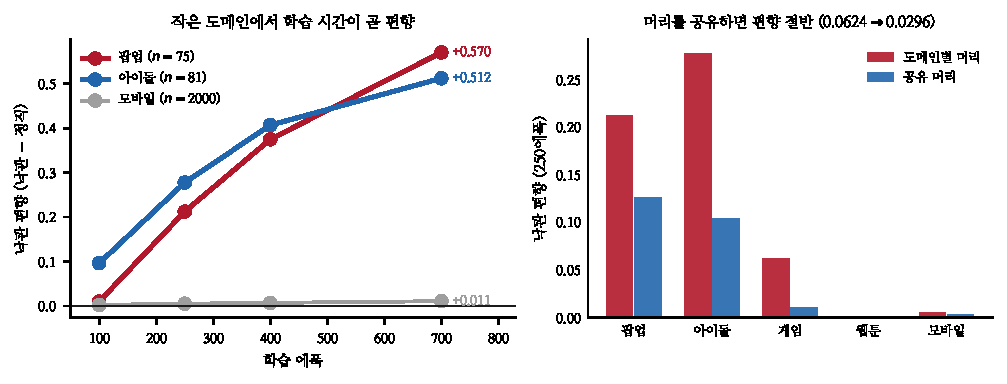
\includegraphics[width=\textwidth]{figs/ep.pdf}
\caption{왼쪽 --- 학습 에폭과 낙관 편향. 오른쪽 --- 머리 구조와 편향.}
\end{figure*}

\section{학습 시간이 곧 편향이다}

\begin{table}[t]
\centering\tsize
\caption{낙관 편향(낙관 $-$ 정직). 도메인별 머리, 3폴드.}
\begin{tabular}{rrrr}
\toprule
에폭 & 팝업(75) & 아이돌(81) & 모바일(2000) \\
\midrule
100 & $+$0.010 & $+$0.096 & $+$0.003 \\
250 & $+$0.212 & $+$0.278 & $+$0.005 \\
400 & $+$0.375 & $+$0.407 & $+$0.007 \\
\textbf{700} & \textbf{$+$0.570} & \textbf{$+$0.512} & $+$0.011 \\
\bottomrule
\end{tabular}
\end{table}

팝업 편향이 57배가 되는 동안 모바일은 3.7배다. \textbf{같은 학습, 같은 인코더인데
75건짜리 도메인만 외운다.}

\claimx{작은 도메인에서 낙관 편향은 학습 시간에 거의 비례한다. 팝업(75건)이
100에폭 $+$0.010에서 700에폭 $+$0.570이고 모바일(2,000건)은 $+$0.003에서
$+$0.011이다. \textbf{에폭 수를 보고하지 않은 신경망 수치는 읽을 수 없다.}}
{에폭 넷만 봤고 학습률 · 정규화를 고정했다. 가중치 감쇠를 세게 하면 곡선이
눕겠지만 그러면 큰 도메인의 성적도 내려갈 것이다 --- 교환을 안 쟀다.}

노트 85 · 86이 400에폭을 썼고 그 지점의 팝업 편향이 $+$0.375다. 노트 87이
다른 실행에서 관측한 $+$0.384와 맞는다 --- \textbf{그 수는 잡음이 아니라
설정의 함수였다.}

\section{도메인별 머리가 절반이다}

\begin{table}[t]
\centering\tsize
\caption{머리 구조와 편향. 250에폭.}
\begin{tabular}{lrr}
\toprule
& 도메인별 머리 & 공유 머리 \\
\midrule
팝업 & $+$0.2124 & $+$0.1259 \\
아이돌 & $+$0.2778 & $+$0.1038 \\
게임 & $+$0.0623 & $+$0.0095 \\
모바일 & $+$0.0052 & $+$0.0027 \\
\midrule
\textbf{평균 편향} & $+$0.0624 & \textbf{$+$0.0296} \\
\textbf{정직 평균} & $+$0.4144 & $+$0.4110 \\
\bottomrule
\end{tabular}
\end{table}

\claimx{편향의 절반은 도메인별 머리에서 나오고, 머리를 공유로 바꾸면 정직 성적을
$+$0.0034만 잃고 편향을 절반으로 줄인다. \textbf{공짜에 가깝다.}}{공유 머리는
도메인마다 다른 축$\to$라벨 관계를 하나로 강제한다. 지금은 손해가 작지만
도메인이 더 이질적이면 커질 것이다.}

남은 절반은 공유 인코더 자체다. 3폴드에서 인코더는 그 도메인의 나머지 3분의 2
라벨을 보므로, 작은 도메인일수록 그 3분의 2가 평가 폴드와 닮아 있다.

\section{프로젝트 전체를 훑었다}

\begin{table}[t]
\centering\tsize
\caption{신경망 수치 재검.}
\begin{tabular}{lll}
\toprule
& 절차 & 판정 \\
\midrule
노트 60--62 전이 & 대상 라벨 제외 & 영향 없음 \\
노트 85 $+$0.3575 & 대상 라벨 제외 & 영향 없음 \\
노트 86 $+$0.3692 & 대상 라벨 제외 & 영향 없음 \\
\textbf{노트 86 ``라벨 씀''} & \textbf{인코더가 라벨 봄} & \textbf{철회(87)} \\
노트 86 과거 16건 & 정직 & 영향 없음 \\
노트 87 $+$0.4144 & 정직 & 유효 \\
\bottomrule
\end{tabular}
\end{table}

전이 수치는 전부 대상 도메인의 라벨 지도를 빼고 학습한다 --- 그것이 이 프로젝트의
기본 규약이었고, 그래서 영향이 없다. \textbf{한 번 어긴 자리가 노트 86의 표
하나였고 그것만 무너졌다.}

\begin{quote}\fontsize{9.5}{11.5}\selectfont
\textbf{규약을 하나 더 둔다.} 도메인 안 성적을 신경망으로 보고할 때는
\textbf{정직 절차}(폴드마다 그 폴드의 라벨을 빼고 학습)로만 내고, 낙관값을 함께
적어 편향을 드러낸다. 에폭 수도 함께 적는다.
\end{quote}

\section{코드에 넣었다}

\texttt{state/masked\_encoder.py} 에 \texttt{honest\_selfr()} 를 넣었다 ---
폴드마다 그 폴드의 라벨을 빼고 학습한 뒤 \texttt{encode()} 로 그 폴드를 투영한다.
기본값은 공유 머리 · 250에폭이다.

\begin{quote}\fontsize{9.0}{11}\selectfont\ttfamily
honest\_selfr(data, folds=3, epochs=250,\\
\hspace*{2em}shared\_head=True)
\end{quote}

노트 65가 진단 코드를 \texttt{state/audit.py} 로 모은 것과 같은 조치다 ---
\textbf{규칙은 사람이 어기고 구조는 안 어긴다.}

\section{한계}

\begin{itemize}[leftmargin=1.1em,itemsep=0.15em]
\item 에폭 넷 · 머리 둘만 봤다. 정규화 · 폭 · 학습률은 안 훑었다.
\item 3폴드라 인코더가 그 도메인의 3분의 2 라벨을 본다. leave-one-out 이면
      편향이 더 줄겠지만 계산이 $n$배다.
\item 공유 머리가 손해를 거의 안 낸다는 것은 지금 열 도메인에서다.
\item 재검을 ``절차가 대상 라벨을 뺐는가''로 판정했다. 다른 종류의 누출은
      안 봤다.
\item 노트 60--62의 수치는 이전 세션의 것이라 코드를 다시 돌려 확인하지 않았다.
\end{itemize}

\section{다음}

\begin{enumerate}[leftmargin=1.1em,itemsep=0.15em]
\item \textbf{제품 도구를 만든다} --- 새 팝업 기획서를 넣으면 백분위와 예상
      구간을 내는 스크립트. 노트 77의 가장 엄격한 규약을 그대로 쓴다.
      모델 쪽 지렛대가 닫혔으므로 남은 것은 쓸 수 있게 만드는 일이다.
\item 정규화를 세게 해 편향 곡선을 눕히고 큰 도메인 손해를 잰다.
\item 노트 60--62를 정직 절차로 다시 돌린다.
\item 팝업 표본 --- 세 노트가 같은 곳을 가리킨다(75 · 86 · 87).
\end{enumerate}

\vspace{0.6em}
\hrule height 0.3pt
\vspace{0.5em}
{\footnotesize
\textbf{참고문헌}\\[0.3em]
Varoquaux, G. (2018). Cross-validation failure: small sample sizes lead to large
error bars. \emph{NeuroImage}, 180, 68--77.\\[0.15em]
Cawley, G. C., Talbot, N. L. C. (2010). On over-fitting in model selection and
subsequent selection bias in performance evaluation. \emph{JMLR}, 11, 2079--2107.\\[0.15em]
Zhang, C. et al. (2017). Understanding deep learning requires rethinking
generalization. \emph{ICLR}.\\[0.15em]
Belkin, M. et al. (2019). Reconciling modern machine-learning practice and the
classical bias--variance trade-off. \emph{PNAS}, 116(32), 15849--15854.\\[0.15em]
Bouthillier, X. et al. (2021). Accounting for variance in machine learning
benchmarks. \emph{MLSys}, 3, 747--769.
}

\end{document}
